% L6a lecture companion. Source hashes and section mapping are in README.md.
% Style files and Cornell seal are copied unchanged from L5c/slides.
% The untitled metabolic-map slide uses the complete approved vector PDF.
% Synchronized September 25, 2026 with the instructor-edited lecture order:
% overview and geometry, stoichiometric matrix, flux bounds, linear program.
\documentclass[aspectratio=169,11pt]{beamer}
\usepackage{vnslides}
\usepackage{tabularx}

\renewcommand{\vnlecturecode}{L6a}
\newcolumntype{Y}{>{\raggedright\arraybackslash}X}
\newcommand{\lecturelink}{https://github.com/varnerlab/CHEME-5800-CourseRepository-Fall-2026/blob/main/weeks/week-06/L6a/CHEME-5800-L6a-Lecture-FluxBalanceAnalysis-Fall-2026.ipynb}
\newcommand{\urealink}{https://github.com/varnerlab/CHEME-5800-CourseRepository-Fall-2026/blob/main/weeks/week-06/L6a/CHEME-5800-L6a-Example-UreaCycle-FluxBalance-Fall-2026.ipynb}
\newcommand{\derivationlink}{https://github.com/varnerlab/CHEME-5800-CourseRepository-Fall-2026/blob/main/weeks/week-06/L6a/CHEME-5800-L6a-Advanced-Derivation-FluxBalanceAnalysis-Fall-2026.ipynb}
\newcommand{\lecturesource}[1]{\note{[Sources]\par
  \href{\lecturelink}{L6a lecture: Metabolic Engineering and Flux Balance Analysis.}\par
  #1\par[/Sources]}}
\newcommand{\mapsource}{\lecturesource{Metabolic Engineering. Original course figure:
  ../figs/Fig-Central-Metabolism/Fig-Central-Metabolism.tex.
  Scientific scope and biochemical sources: ../figs/Fig-Central-Metabolism/README.md.
  Selected connections in central metabolism.}}

\title{\texorpdfstring{{\vnheavy L6a}}{L6a}: Metabolic Engineering and Flux Balance Analysis}
\subtitle{\texorpdfstring{Stoichiometry, reaction bounds, and production limits\\[3pt]CHEME 5800 Cornell University}{Stoichiometry, reaction bounds, and production limits; CHEME 5800 Cornell University}}
\author{Copyright Jeffrey Varner 2026. All Rights Reserved}

\begin{document}
\special{pdf:minorversion 7}
\vntitlepage

% Introduction and learning objectives.
\begin{frame}{Objectives for Today}
  How do material balances and biological constraints limit the production
  of a desired compound?

  \vspace{0.4em}
  {\large\textbf{\ink{Today's concepts}}}
  \vspace{0.2em}
  \begin{itemize}\setlength{\itemsep}{0.7em}
    \item You will \hilite{represent a metabolic reaction network as a
      stoichiometric matrix} and interpret its rows, columns, and coefficient signs.
    \item You will \hilite{formulate the flux balance analysis problem}, a linear
      program for the unknown fluxes, and explain its objective and the
      constraints that define the feasible solution space.
    \item You will \hilite{develop and interpret flux bounds} from reaction
      reversibility and enzyme capacity, and explain their biological meaning.
  \end{itemize}
  \slidenote{Lecture:}{\href{\lecturelink}{Metabolic Engineering and Flux Balance Analysis}}
  \lecturesource{Introduction and Learning Objectives.}
\end{frame}

% Examples. Computational setup stays in the companion notebooks.
\begin{frame}{Lecture and Examples}
  \textbf{\ink{Lecture:}}
  \href{\lecturelink}{Metabolic Engineering and Flux Balance Analysis}

  In this lecture, we introduce flux balance analysis (FBA), a tool based on
  linear programming, to estimate reaction rates (called fluxes) in a metabolic
  network.

  \vspace{1.0em}
  \textbf{\ink{Example:}}
  \href{\urealink}{Calculate fluxes in a urea-cycle model}

  In this example, we build a stoichiometric model of the urea cycle in human
  cells, estimate reaction directions and enzyme capacities to establish the
  flux bounds, and solve a linear program to maximize urea export. The same
  approach applies to any metabolic network.

  \vspace{0.9em}
  We can explore the connections among metabolic pathways in the
  \href{https://www.kegg.jp/pathway/map01100}{KEGG metabolic pathways map}.
  \lecturesource{Introduction and Examples: urea-cycle example and KEGG map01100.}
\end{frame}

% A single untitled network overview introduces metabolic engineering.
\begin{frame}[plain]
  \centering
  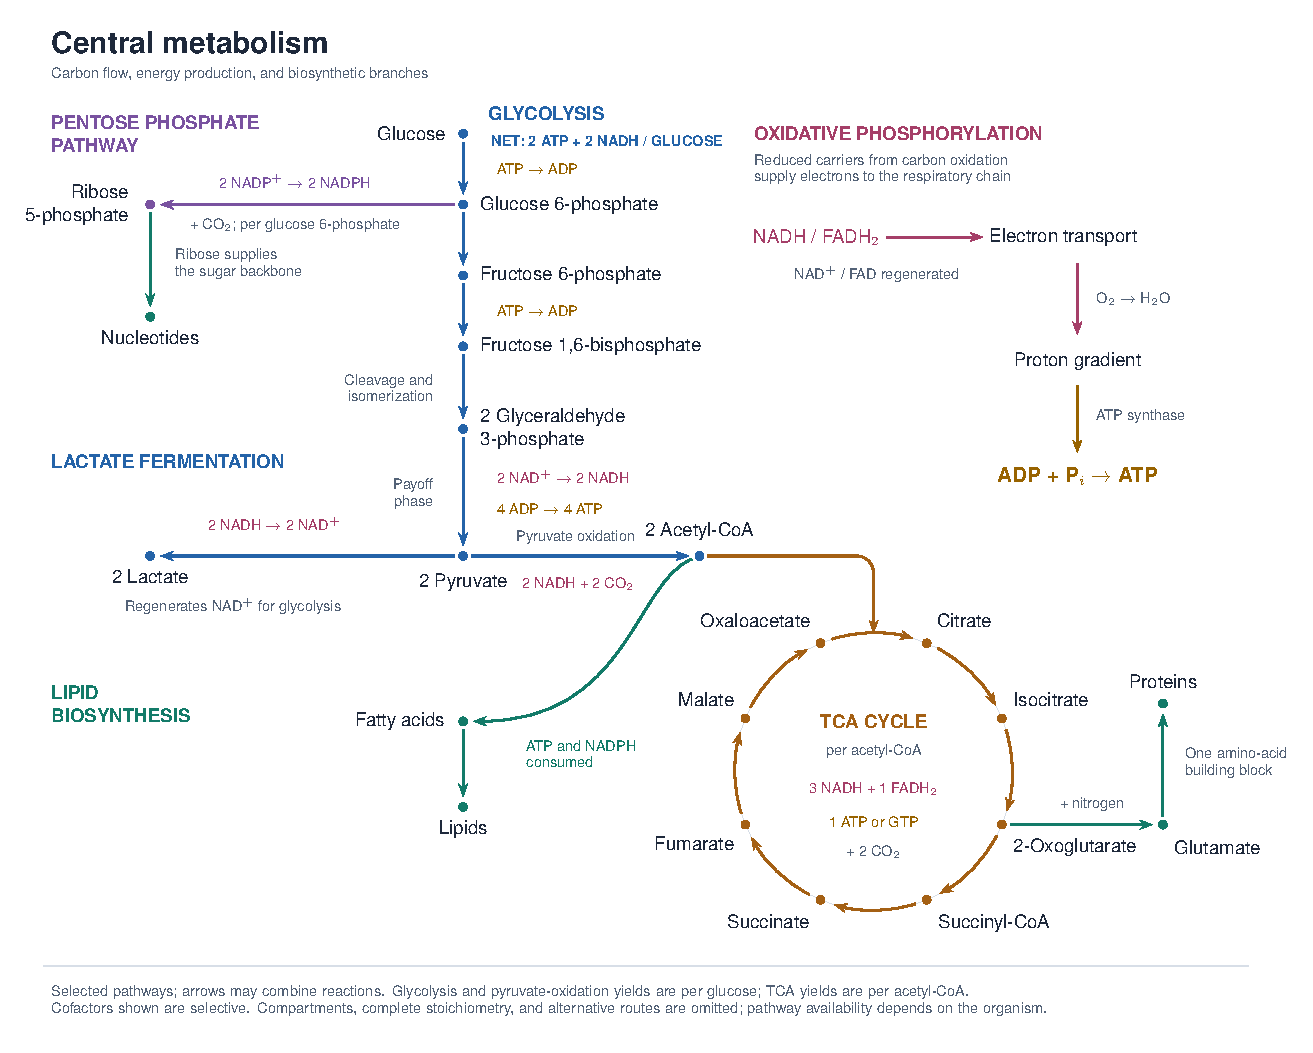
\includegraphics[width=\textwidth,height=0.94\paperheight,keepaspectratio]{assets/Fig-Central-Metabolism.pdf}
  \mapsource
\end{frame}

\begin{frame}{What Is Metabolic Engineering?}
  Metabolic pathways encode the enzyme-catalyzed reactions that convert
  nutrients into biomass and energy. Some pathways are highly conserved across
  species, such as \hilite{central metabolism}: glycolysis, the pentose
  phosphate pathway, and the TCA cycle.

  \vspace{0.8em}
  \hilite{Metabolic engineering} is the directed modification of an
  organism's metabolic pathways through genetic and regulatory changes
  to increase production of a desired compound or to enable new products.

  \vspace{0.8em}
  The engineering question is: how can we redirect carbon, nitrogen, and
  energy toward a target molecule while meeting the cell's other requirements?
  We describe the flow of material using \hilite{metabolic fluxes}: reaction
  rates per unit volume or biomass.

  \slidenote{Early work:}{\href{https://pubmed.ncbi.nlm.nih.gov/2047876/}{Bailey (1991)};
    \href{https://pubmed.ncbi.nlm.nih.gov/1904627/}{Stephanopoulos and Vallino (1991)}.}
  \lecturesource{Metabolic Engineering: pathways, definition, engineering question, and fluxes.
    Bailey, Science 252, 1668–1675 (1991).
    Stephanopoulos and Vallino, Science 252, 1675–1681 (1991).}
\end{frame}

% Flux Balance Analysis: definition, then the geometry figure.
\begin{frame}{Flux Balance Analysis}
  \hilite{Flux balance analysis (FBA)} estimates optimal metabolic reaction
  rates (fluxes) from material balances and biological constraints.

  \vspace{0.8em}
  FBA uses linear programming to find the flux distribution that optimizes a
  chosen objective function, subject to stoichiometric and capacity constraints,
  at a \hilite{pseudo-steady state}.

  \vspace{0.8em}
  \begin{enumerate}\setlength{\itemsep}{0.7em}
    \item The \hilite{stoichiometric matrix} encodes the reaction network and
      the steady-state material balances.
    \item The \hilite{flux bounds} restrict each reaction rate using
      reversibility and enzyme capacity.
    \item The \hilite{linear program} combines the balances, bounds, and an
      objective, such as maximizing product export.
  \end{enumerate}
  \lecturesource{Flux Balance Analysis: definition and components.}
\end{frame}

\begin{frame}{Conservation, Bounds, and Alternate Optima}
  \centering
  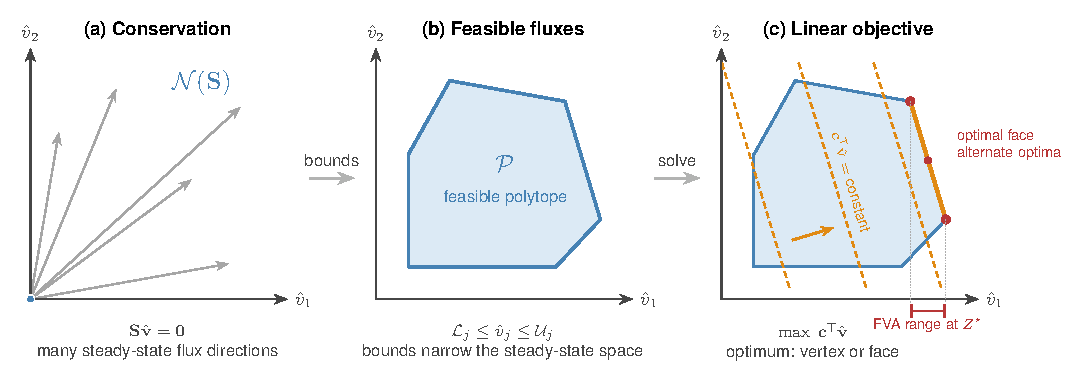
\includegraphics[width=\textwidth,height=0.68\paperheight,keepaspectratio]{assets/Fig-FBA-FeasibleSpace.pdf}

  \vspace{0.4em}
  \raggedright
  Balances define the null space, bounds cut it to the feasible set $\mathcal P$,
  and the objective selects an edge, so the optimum is \hilite{not unique}.
  \hilite{Flux variability analysis} finds the range of each flux at $Z^\star$.
  \lecturesource{Flux Balance Analysis: geometry figure and caption.
    Figure: ../figs/Fig-FBA-FeasibleSpace, adapted from the Varner lab chapter
    linear-program geometry figure.}
\end{frame}

% Stoichiometric matrix, from a metabolic reconstruction.
\begin{frame}{Stoichiometric Matrix}
  We build $\mathbf S$ from a \hilite{metabolic reconstruction}: a curated set of
  reactions, metabolites, and stoichiometric coefficients.
  Let $\mathcal M$ be the set of modeled species and $\mathcal R$ the set of
  reactions. The entry $\sigma_{ij}$ is the net coefficient of species $i$
  in reaction $j$:
  \[
    \mathbf S=[\sigma_{ij}]
      \in\mathbb R^{|\mathcal M|\times|\mathcal R|}.
  \]

  \begin{itemize}\setlength{\itemsep}{0.3em}
    \item One \hilite{column} describes a reaction; one \hilite{row}
      collects contributions to a species balance.
    \item $\sigma_{ij}>0$: species $i$ is a \hilite{product} of reaction $j$.
      $\sigma_{ij}<0$: species $i$ is a \hilite{reactant}.
    \item $\sigma_{ij}=0$: species $i$ is not involved, or the net stoichiometry is zero.
  \end{itemize}

  \vspace{0.2em}
  The matrix records net stoichiometry. Regulation enters through the flux
  bounds, not the stoichiometric matrix.
  \lecturesource{Stoichiometric Matrix: reconstruction, definition, and coefficient signs.}
\end{frame}

\begin{frame}{Biological Data Resources}
  \renewcommand{\arraystretch}{1.45}
  \setlength{\tabcolsep}{5pt}
  \begin{tabularx}{\textwidth}{@{}lY@{}}
    \toprule
    Resource & What we use it for\\
    \midrule
    \href{https://academic.oup.com/nar/article/53/D1/D672/7824602}{KEGG} & We examine pathways and connections among genes, enzymes, and reactions.\\
    \href{https://pubmed.ncbi.nlm.nih.gov/29447345/}{BioCyc} & We find pathway and genome information for a particular organism.\\
    \href{https://academic.oup.com/nar/article/48/D1/D402/5614178}{BiGG Models} & We obtain metabolic models with standardized metabolite and reaction identifiers.\\
    \href{https://academic.oup.com/nar/article/49/D1/D498/5992283}{BRENDA} & We find enzyme properties and kinetic measurements to estimate flux bounds.\\
    \href{https://academic.oup.com/nar/article/38/suppl_1/D750/3112244}{BioNumbers} & We find measured biological quantities and their literature sources.\\
    \bottomrule
  \end{tabularx}
  \slidenote{Readings:}{Resource names link to the papers listed in the lecture.}
  \lecturesource{Stoichiometric Matrix: five-resource table.
    Kanehisa et al. (2025); Karp et al. (2019); Norsigian et al. (2020);
    Chang et al. (2021); Milo et al. (2010). Linked papers in the table.}
\end{frame}

\begin{frame}{Example: One Reaction Gives One Column}
  \centering
  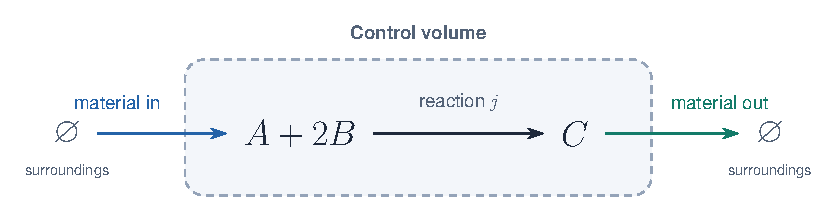
\includegraphics[width=0.62\textwidth,height=0.40\paperheight,keepaspectratio]{assets/Fig-Stoichiometric-ControlVolume.pdf}

  \raggedright
  The dashed boundary encloses the modeled species; material enters and leaves
  through it. Reaction $j$ consumes one unit of $A$ and two units of $B$ to
  produce one unit of $C$. With rows ordered $(A,B,C)$:
  \[
    A+2B\longrightarrow C,
    \qquad
    \mathbf s_j=\begin{bmatrix}-1\\-2\\1\end{bmatrix},
    \qquad
    \mathbf s_j\hat v_j=\begin{bmatrix}-\hat v_j\\-2\hat v_j\\\hat v_j\end{bmatrix}.
  \]
  The coefficient $-2$ means $B$ is consumed at twice the reaction flux. A
  negative flux reverses the signs; the column stays the same.
  \lecturesource{Stoichiometric Matrix, Example: Stoichiometric Column.
    Figure: ../figs/Fig-Stoichiometric-ControlVolume.}
\end{frame}

\begin{frame}{Exchange Reactions Cross the Boundary}
  An \hilite{exchange reaction} connects a metabolite to the surroundings,
  written $\emptyset$, which we do not balance. Its column has a single
  nonzero entry. For the reactant $A$ supplied by exchange reaction $k$:
  \[
    \emptyset\longrightarrow A,
    \qquad
    \mathbf s_k=\begin{bmatrix}1\\0\\0\end{bmatrix}.
  \]

  \vspace{0.5em}
  A positive flux brings $A$ into the control volume; a negative flux removes it.
  The urea example writes every exchange this way. The BiGG models in the L6b
  lab write $A\longrightarrow\emptyset$, so uptake is negative there.

  \vspace{0.6em}
  The sign convention does not affect the FBA solution, but it does affect the
  interpretation of the fluxes.
  \lecturesource{Stoichiometric Matrix: exchange reactions and sign conventions.}
\end{frame}

% A model for flux bounds: retain the instructor's brace notation.
\begin{frame}{A Model for Flux Bounds}
  Flux bounds are \hilite{integrative}: they bring many types of genetic and
  biochemical information into the problem. For enzyme-catalyzed reaction $j$,
  a general model for the bounds is:
  \[
    \underbrace{
      -\delta_j\overbrace{
        \left[V_{max,j}^{\circ}\left(\frac{e}{e^{\circ}}\right)
        \theta_j(\dots)f_j(\dots)\right]
      }^{\text{reverse: other functions or parameters?}}
    }_{\mathcal L_j}
    \leq\hat v_j\leq
    \underbrace{
      V_{max,j}^{\circ}\left(\frac{e}{e^{\circ}}\right)
      \theta_j(\dots)f_j(\dots)
    }_{\mathcal U_j}.
  \]

  \vspace{0.8em}
  Here $V_{max,j}^{\circ}$ is the maximum reaction velocity at a characteristic
  enzyme abundance, $e/e^{\circ}$ corrects for the actual abundance, $\theta_j$
  is the allosteric activity, $f_j$ the substrate saturation, and $\delta_j$
  the reversibility parameter.

  \vspace{0.6em}
  This model assumes equal forward and reverse capacities for a reversible
  reaction. We fix every quantity \hilite{before solving} the linear program.
  \lecturesource{A Model for Flux Bounds: annotated bound model and integrative role.}
\end{frame}

\begin{frame}{Reference Enzyme Capacity}
  Let $k_{cat,j}^{\circ}$ be the reference catalytic turnover number and
  $e^{\circ}$ the characteristic enzyme abundance. The reference capacity is:
  \[
    V_{max,j}^{\circ}=k_{cat,j}^{\circ}e^{\circ}.
  \]

  \vspace{0.4em}
  \renewcommand{\arraystretch}{1.35}
  \setlength{\tabcolsep}{5pt}
  \begin{tabularx}{\textwidth}{@{}lYl@{}}
    \toprule
    Quantity & Meaning & Units\\
    \midrule
    $V_{max,j}^{\circ}$ & This is the maximum rate at reference enzyme abundance. & $\mathrm{mmol\,gDW^{-1}\,h^{-1}}$\\
    $k_{cat,j}^{\circ}$ & This is the turnover rate at substrate saturation. & $\mathrm{h^{-1}}$\\
    $e^{\circ},\ e$ & $e^{\circ}$ and $e$ denote reference and actual abundance. & $\mathrm{mmol\,gDW^{-1}}$\\
    \bottomrule
  \end{tabularx}

  \vspace{0.4em}
  The ratio $e/e^{\circ}$ scales the reference capacity to the actual
  abundance of the enzyme catalyzing reaction $j$.
  \lecturesource{A Model for Flux Bounds: maximum-velocity equation and nomenclature table.}
\end{frame}

\begin{frame}{Activity, Saturation, and Reversibility}
  The activity factor $\theta_j$, saturation factor $f_j$, and reversibility parameter $\delta_j$ are dimensionless:

  \vspace{0.6em}
  \renewcommand{\arraystretch}{1.6}
  \setlength{\tabcolsep}{5pt}
  \begin{tabularx}{\textwidth}{@{}lY@{}}
    \toprule
    Quantity & Meaning\\
    \midrule
    $\theta_j(\dots)\in[0,1]$ & The activity factor gives the fraction of maximal activity available under allosteric regulation.\\
    $f_j(\dots)\in[0,1]$ & The saturation factor describes substrate availability. A value of one represents saturating substrates.\\
    $\delta_j\in\{0,1\}$ & The reversibility parameter is zero for a forward-only reaction and one when reverse flux is allowed.\\
    \bottomrule
  \end{tabularx}

  \vspace{0.8em}
  Activity and substrate availability can reduce the capacity below
  $V_{max,j}^{\circ}(e/e^{\circ})$.
  \lecturesource{A Model for Flux Bounds: nomenclature for theta, f, and delta.}
\end{frame}

\begin{frame}{Simplified Bounds Model}
  Let's assume $e/e^{\circ}\sim1$, no allosteric inputs $\theta_j(\dots)\sim1$,
  and saturating substrates $f_j(\dots)\sim1$. Then the flux bounds are:
  \[
    \underbrace{-\delta_j V_{max,j}^{\circ}}_{\mathcal L_j}
      \leq\hat v_j\leq
    \underbrace{V_{max,j}^{\circ}}_{\mathcal U_j}.
  \]

  \vspace{0.5em}
  \begin{itemize}\setlength{\itemsep}{0.8em}
    \item For a \hilite{forward-only reaction}, $\delta_j=0$, so the flux satisfies
      $0\leq\hat v_j\leq V_{max,j}^{\circ}$.
    \item For a \hilite{reversible reaction}, $\delta_j=1$, so the flux satisfies
      $-V_{max,j}^{\circ}\leq\hat v_j\leq V_{max,j}^{\circ}$.
  \end{itemize}

  \vspace{0.7em}
  The bounds are a function of the maximum reaction velocity, the turnover
  number, and our assumed characteristic enzyme abundance.
  \lecturesource{Simplified bounds model: assumptions, bound equation, and interpretation.}
\end{frame}

\begin{frame}{Exchange Bounds Specify the Surroundings}
  Exchange bounds limit nutrient uptake and product secretion. In the urea
  example, we write every exchange as uptake from the surroundings,
  so \hilite{positive flux represents uptake} and negative flux represents export.

  \vspace{0.7em}
  \begin{itemize}\setlength{\itemsep}{0.8em}
    \item The upper bound limits the uptake rate.
    \item An upper bound of zero prevents uptake through that reaction.
    \item A negative lower bound sets the largest allowed export rate.
    \item A lower bound of zero prevents export through that reaction.
  \end{itemize}

  \vspace{0.7em}
  The exchange bounds specify which nutrients the system can take up and
  which products it can release. Internal reactions have separate bounds
  based on enzyme capacity and reaction direction.
  \lecturesource{Urea-cycle example, Step 3: exchange bounds under the uptake-positive convention.}
\end{frame}

% Linear programming formulation: assumptions, boxed LP, and objective convention.
\begin{frame}{The Flux Balance Approximation}
  The FBA problem has the same structure as the minimum-cost flow problem:
  $\mathbf S$ plays the role of the incidence matrix, and the exchange
  reactions are the sources and sinks.

  \vspace{0.6em}
  The material balances rest on two assumptions:
  \begin{itemize}\setlength{\itemsep}{0.5em}
    \item The amount of each metabolite per gram of biomass stays constant.
    \item Growth dilution is small compared with production and consumption.
  \end{itemize}

  \vspace{0.4em}
  Then, for each species $i\in\mathcal M$:
  \[
    \sum_{j\in\mathcal R}\sigma_{ij}\hat v_j=0,
    \qquad\text{or}\qquad
    \mathbf S\hat{\mathbf v}=\mathbf 0.
  \]
  \slidenote{Derivation:}{\href{\derivationlink}{Flux balance analysis material balances}}
  \lecturesource{Linear Programming Formulation: analogy and assumptions.
    \href{\derivationlink}{Companion derivation notebook.}}
\end{frame}

\begin{frame}{Flux Balance Analysis Problem}
  Let $c_j$ be the objective weight of reaction $j$, and let
  $\mathcal L_j$ and $\mathcal U_j$ be its flux bounds.
  With the coefficients, weights, and bounds fixed, we solve:
  {\small
  \[
    \boxed{
    \begin{aligned}
      \underset{\hat v_1,\hat v_2,\ldots,\hat v_{|\mathcal R|}}{\operatorname{maximize}}\quad
        &\sum_{j\in\mathcal R}c_j\hat v_j\\[3pt]
      \text{subject to}\quad
        &\sum_{j\in\mathcal R}\sigma_{ij}\hat v_j=0,
          &&i\in\mathcal M\quad\text{(material balance constraints)}\\[3pt]
        &\mathcal L_j\leq\hat v_j\leq\mathcal U_j,
          &&j\in\mathcal R\quad\text{(thermodynamics and kinetic constraints)}
    \end{aligned}}
  \]}
  A \hilite{feasible} distribution satisfies all balances and bounds.
  The objective selects an \hilite{optimal} distribution from the feasible set;
  the optimal solution may \hilite{not be unique}.
  \lecturesource{Linear Programming Formulation: boxed FBA problem and interpretation.}
\end{frame}

\begin{frame}{An Objective for Product Export}
  Let $p$ denote the urea exchange reaction, \texttt{b4}. We write this reaction
  as uptake from the surroundings, so \hilite{negative flux represents export}.
  We set its objective weight to $-1$ and all other weights to zero:
  \[
    c_j=\begin{cases}-1,&j=p,\\0,&j\neq p,\end{cases}
    \qquad
    \sum_{j\in\mathcal R}c_j\hat v_j=-\hat v_p.
  \]

  \vspace{0.5em}
  Maximizing $-\hat v_p$ makes the urea exchange flux as negative as the
  balances and bounds allow, which maximizes urea export.

  \vspace{0.7em}
  We express metabolic fluxes in $\mathrm{mmol\,gDW^{-1}\,h^{-1}}$,
  where gDW means grams of dry biomass. Each bound has the units of its flux.
  \lecturesource{Urea-cycle example, Step 4: uptake-positive exchange convention,
    urea-export objective, and flux units.}
\end{frame}

\begin{frame}{Example: Calculate Fluxes in a Urea-Cycle Model}
  In this example, we calculate the maximum urea export rate for a
  urea-cycle network in human cells.

  \vspace{0.7em}
  \begin{enumerate}\setlength{\itemsep}{0.7em}
    \item We build the stoichiometric matrix, species and reaction lists, and
      default bounds from the network file.
    \item We assign reaction directions from Gibbs energy estimates and set
      enzyme capacities from turnover numbers and a reference enzyme abundance.
    \item We solve the linear program, inspect the optimal fluxes, and check the
      solution against the balances and bounds.
  \end{enumerate}

  \vspace{0.7em}
  The same approach applies to any metabolic network, and the bounds show how
  many types of biochemical information integrate into one problem.
  \slidenote{Example:}{\href{\urealink}{Calculate fluxes in a urea-cycle model}}
  \lecturesource{Linear Programming Formulation: urea-cycle example callout.
    \href{\urealink}{Companion urea-cycle example.}}
\end{frame}

% Summary: opening, exactly three takeaways, and the closing lesson.
\begin{frame}{Summary}
  We formulated flux balance analysis as a linear program, combining a
  metabolic network, biological constraints, and a production objective.

  \vspace{0.5em}
  {\large\textbf{\ink{Key takeaways}}}
  \vspace{0.3em}
  \begin{itemize}\setlength{\itemsep}{0.9em}
    \item \textbf{\ink{Stoichiometric matrix.}} Rows are metabolites, columns are
      reactions, entries are net stoichiometric coefficients.
    \item \textbf{\ink{Flux balance analysis.}} A linear program for the unknown
      fluxes: a production objective, subject to balances and bounds.
    \item \textbf{\ink{Flux bounds.}} Turnover number times enzyme abundance;
      they integrate biochemical information into the problem.
  \end{itemize}

  \vspace{0.8em}
  FBA lets us predict how network changes affect production of a desired compound.
  \lecturesource{Summary: opening, three key takeaways, and closing lesson.}
\end{frame}

\end{document}
